\documentclass[aspectratio=169]{beamer}
\usepackage[no-math,deluxe]{luatexja-preset}
\renewcommand{\kanjifamilydefault}{\gtdefault}
\usepackage{minted}
\usepackage{xcolor}
\usepackage{hyperref}
\usepackage{amsmath}
\setbeamertemplate{navigation symbols}{}

\title{テスト駆動開発 ハンズオン \#2}
\subtitle{Test-Driven Development Hands-On \#2}
\author{ASUKA Y}
\date{Oct 2 2022}

\begin{document}

\begin{frame}
  \titlepage
\end{frame}

\section*{INDEX}
\begin{frame}
  \frametitle{テスト駆動開発ハンズオン \#2}
  \tableofcontents
\end{frame}

\section{\#1のおさらい}
\subsection{テスト駆動開発とは何か}
\begin{frame}\frametitle{テスト開発とは何か}
  \begin{quote}
    テスト駆動開発(TDD)はテスト技法ではない...
    TDDは分析技法であり、設計技法であり、
    実際には開発のすべてのアクティビティを構造化する技法なのだ。
  \end{quote}
  \begin{flushright}
    ---Kent Beck
  \end{flushright}

  テスト技法ではなく、開発技法である。

  {
    \large \color{blue}
    $\rightarrow$
    テストを書くことが目的ではない。
  }
\end{frame}

\subsection{テスト駆動開発が目指すもの}
\begin{frame}\frametitle{テスト駆動開発が目指すもの}
  \begin{quote}
    「動作するきれいなコード」。
    Ron Jeffiresのこの簡潔な言葉が、
    テスト駆動開発(TDD)のゴールだ。
    動作するきれいなコードはあらゆる意味で価値がある。
  \end{quote}
  \begin{flushright}
    ---Kent Beck
  \end{flushright}

  TDDは動作する「きれいなコード」に辿り着くために、
  {\color{blue} 自動化されたテストによって開発を推し進める技法}である。
\end{frame}

\begin{frame}[fragile]\frametitle{動作するきれいなコード}
  \begin{itemize}
    \item {\color{blue} 開発が予測可能になる。}
      何が完成していて、何が完成していないかがわかる。
    \item {\color{blue} コードが伝えようとしていることを余すところなく受け取れる。}
      最初に思いついたコードを書き殴っただけで終わりなら、
      再考してより良いコードを書くチャンスは永遠に来ない。

    \color{blue}
    \item あなたが作るソフトウェアのユーザを快適にする。
    \item チームメイトはあなたを信頼し、あなたもまたチームメイトを信頼する。
    \item 書いていて気持ちがいい。
  \end{itemize}
\end{frame}

\subsection{テスト駆動開発の進め方}
\begin{frame}\frametitle{テスト駆動開発の進め方}
  \begin{enumerate}
    \item まずはテストを1つ書く
    \item すべてのテストを走らせ、新しいテストの失敗を確認する
    \item 小さな変更を行う
    \item すべてのテストを走らせ、すべて成功することを確認する
    \item リファクタリングを行って重複を排除する
  \end{enumerate}

  \begin{center}
    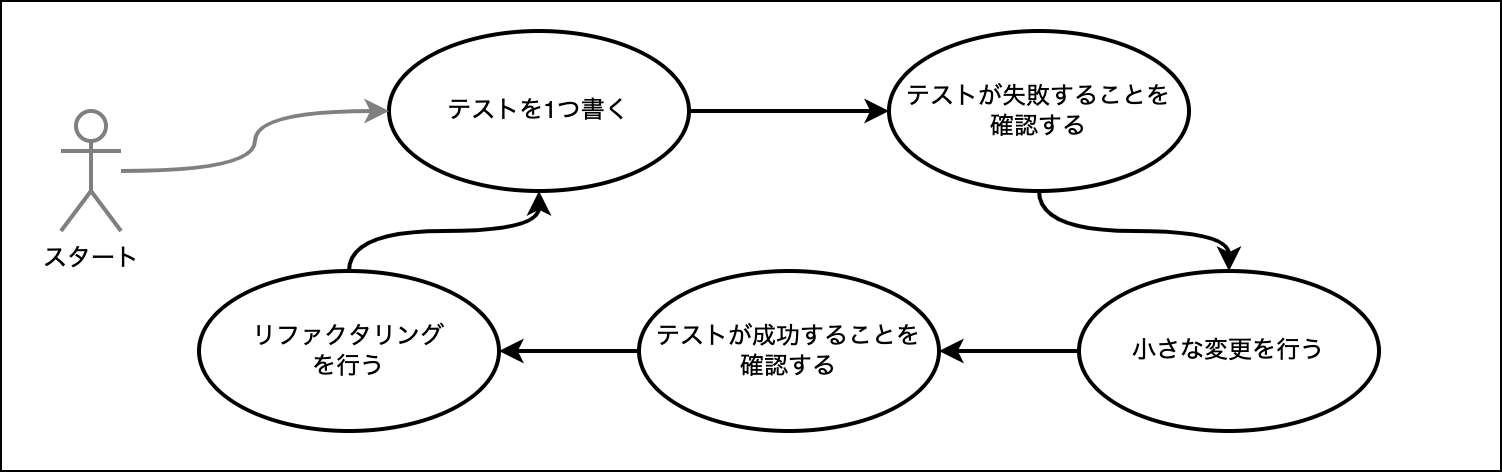
\includegraphics[height=4cm]{asset/tdd_cycle.png}
  \end{center}
\end{frame}

\begin{frame}\frametitle{\#1の資料置き場}
  \url{https://github.com/a-skua/tdd-handson/releases/tag/vol.1}
\end{frame}

\section{ハンズオン}
\subsection{ライフゲーム}
\begin{frame}\frametitle{ライフゲームとは何か}
  \begin{quote}
    ライフゲームは1970年にイギリスの数学者ジョン・ホートン・コンウェイが考案した生命の誕生、進化、淘汰などのプロセスを簡易的なモデルで再現したシミュレーションゲームである。

    生物集団においては、過疎でも過密でも個体の生存に適さないという個体群生態学的な側面を背景に持つ。セル・オートマトンのもっともよく知られた例でもある。
  \end{quote}
  \begin{flushright}
    ---
    \href{https://ja.wikipedia.org/wiki/\%E3\%83\%A9\%E3\%82\%A4\%E3\%83\%95\%E3\%82\%B2\%E3\%83\%BC\%E3\%83\%A0}{ライフゲーム Wikipedia}
  \end{flushright}
\end{frame}

\begin{frame}\frametitle{ライフゲームのルール}
  \begin{center}
    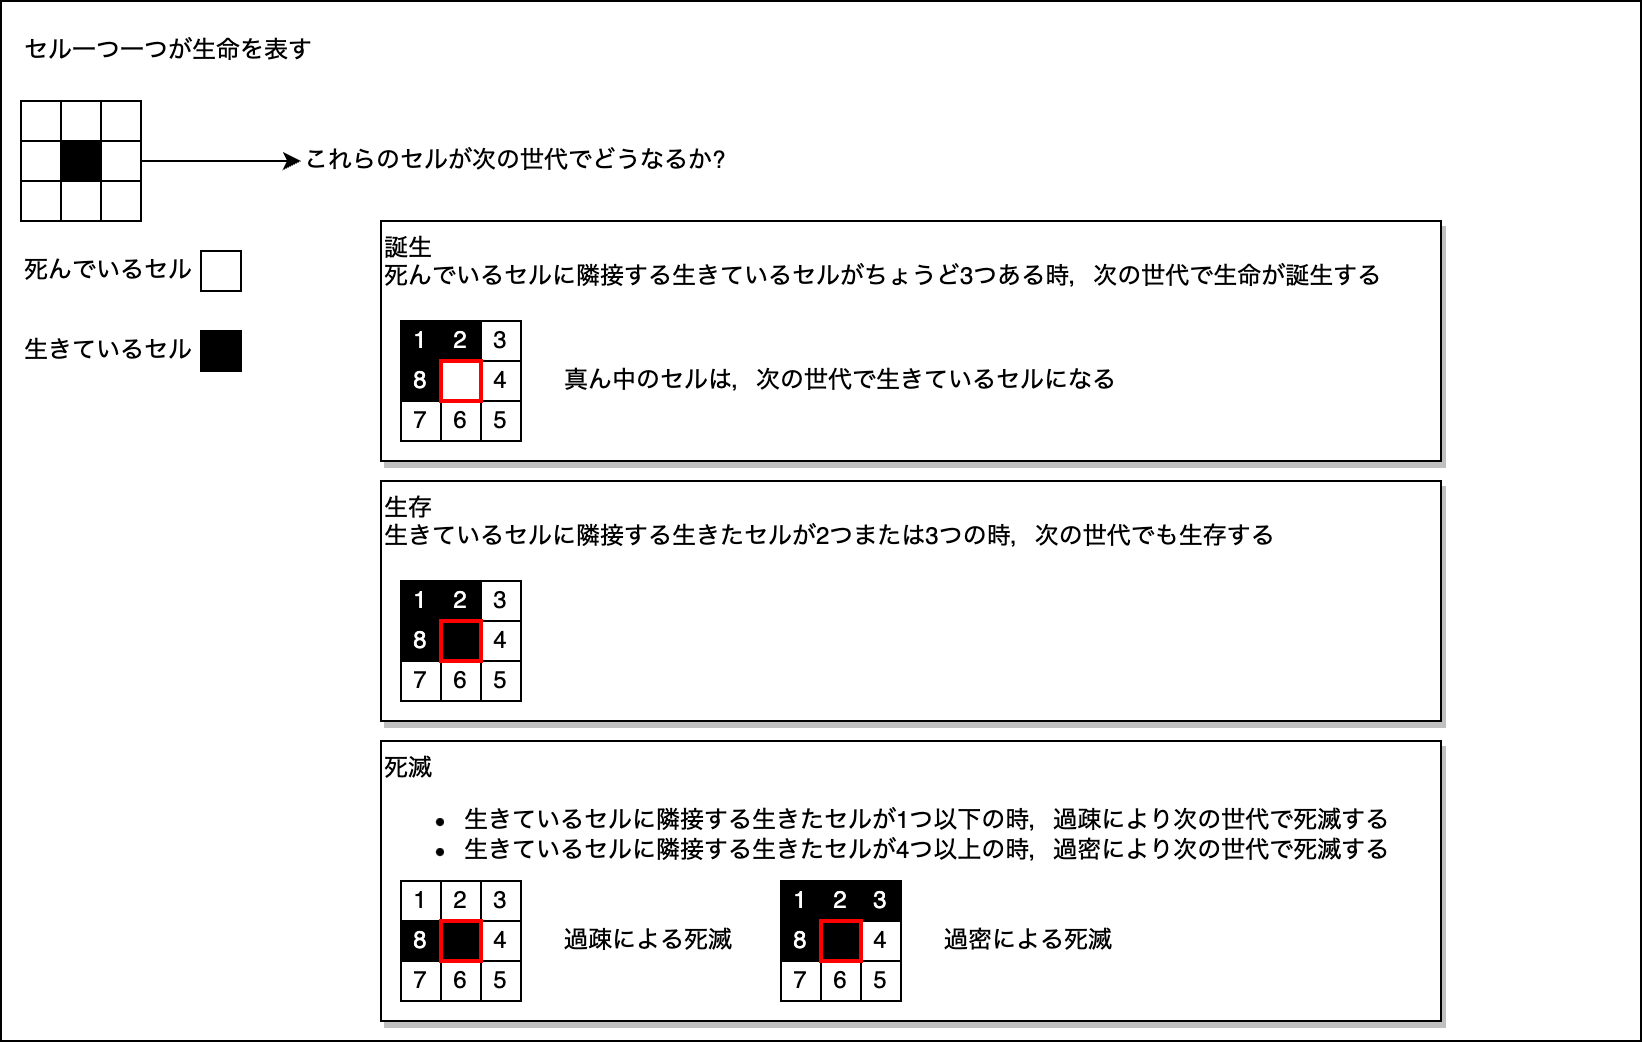
\includegraphics[height=7.5cm]{asset/lifegame.png}
  \end{center}
\end{frame}

\begin{frame}\frametitle{ライフゲームのルール}
  \begin{center}
    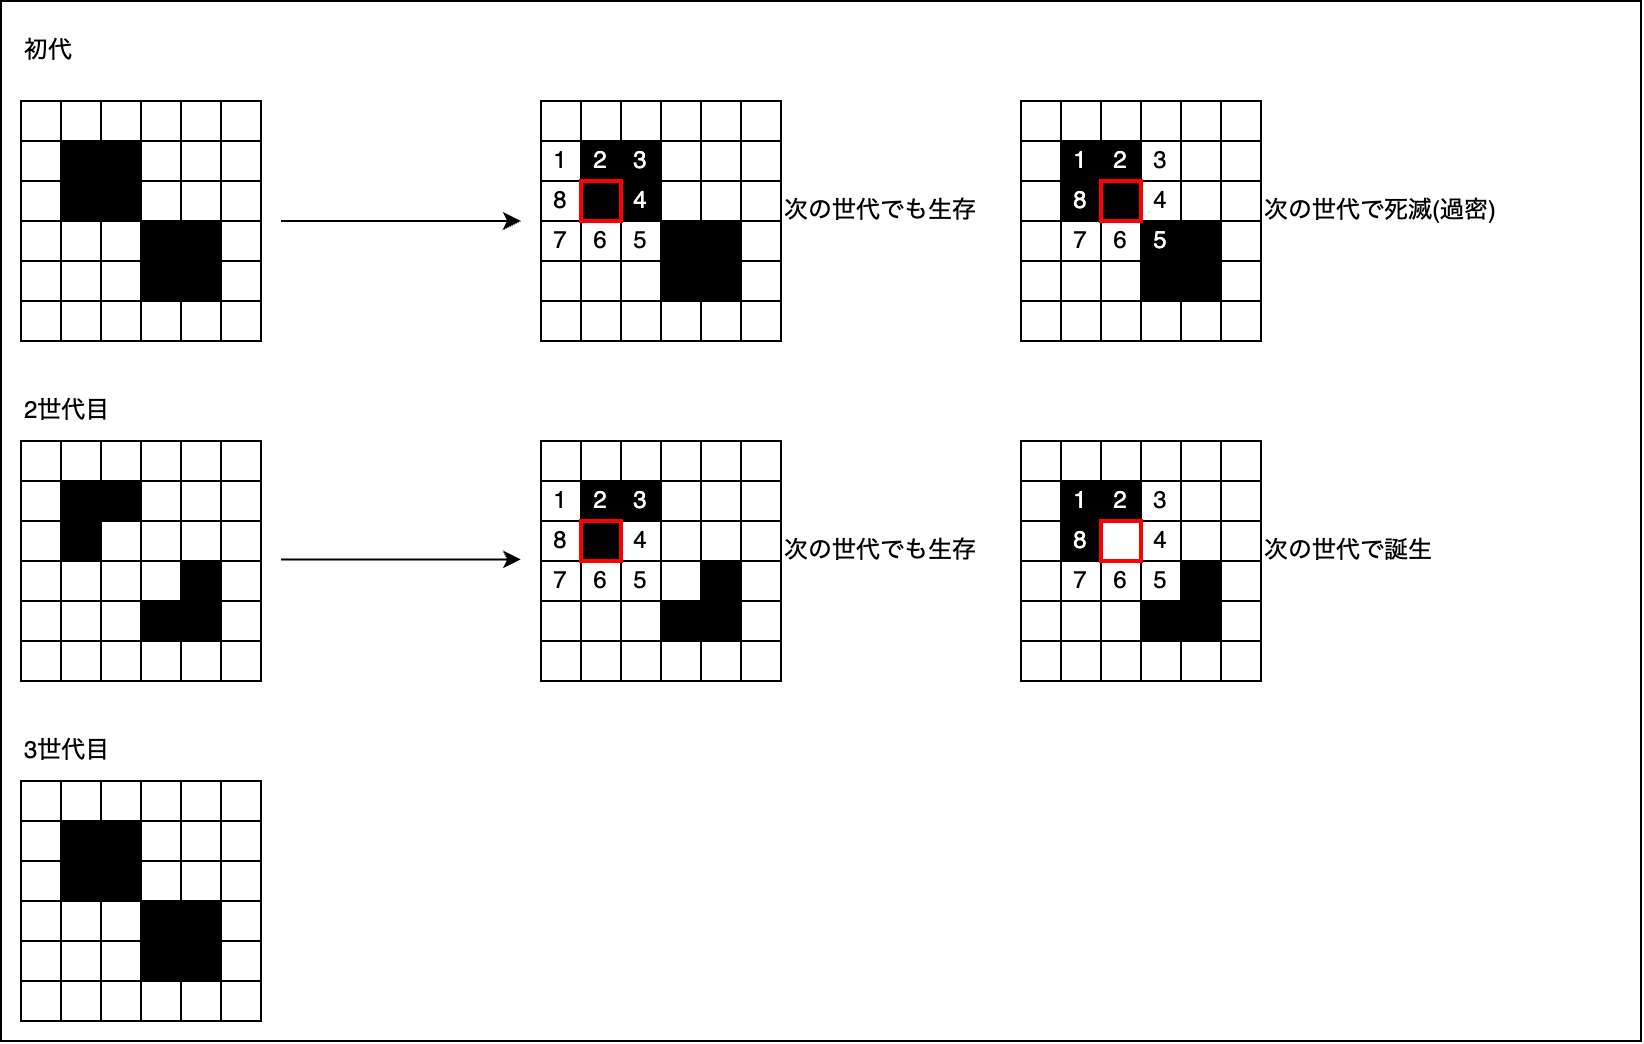
\includegraphics[height=7.5cm]{asset/lifegame_cycle.png}
  \end{center}
\end{frame}

\begin{frame}\frametitle{ライフゲームをプログラムに落とし込むためにやるべきこと}
  \begin{enumerate}
    \item 現在のを設定する(初期化)
    \item 次の世代の状態を決定する(誕生するのか? 生存するのか? 死滅するのか?)
    \item 世代を更新する
  \end{enumerate}

  どう実装するか,書き始める前に方針を考えてみましょう
\end{frame}

\begin{frame}\frametitle{実装例}
  \url{https://github.com/a-skua/lifegame-ts}
\end{frame}

\begin{frame}\frametitle{ハンズオンの成果物}
  \url{https://github.com/a-skua/lifegame-go}
\end{frame}
\end{document}
